\begin{scanpage}{0125}{108}
\noindent\begin{minipage}[t]{.42\linewidth}\vspace{0pt}\centering
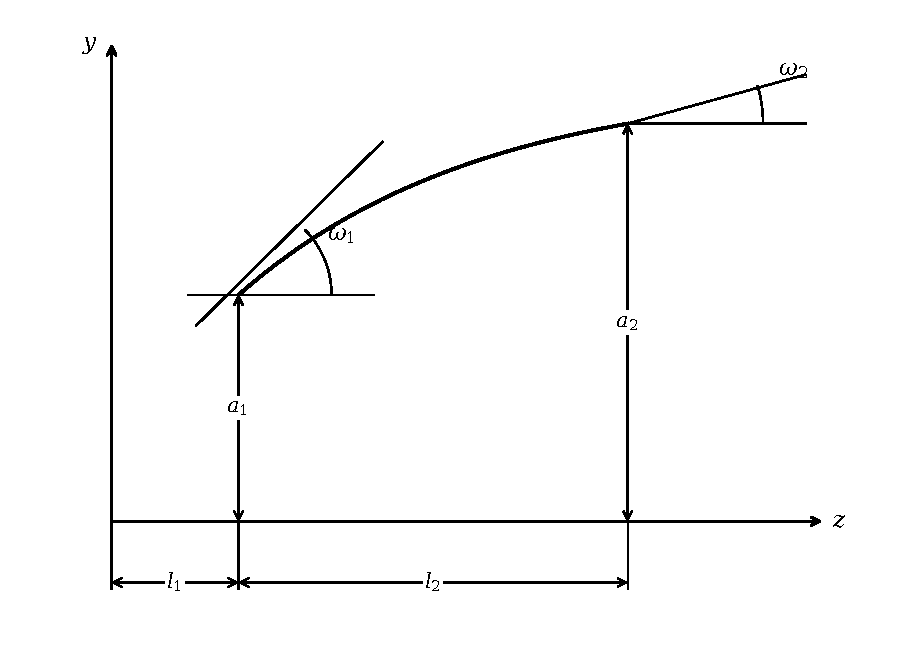
\includegraphics[width=.9\linewidth]{images/recreated/b-0125-fig40.pdf}

\raggedright Figure 40. The generatrix of the lateral surface of a truncated paraboloid of rotation.
\end{minipage}\hfill\begin{minipage}[t]{.54\linewidth}\vspace{0pt}
\sectiontitle{19}{A Spherical Surface}
Incident wave (16.20) excites a surface current on the surface of an ideally conducting sphere (a radius of $\rho$ and a center on the $z$ axis at the point $z=\rho$). The uniform part of this current has the components
\[\left.\begin{aligned}j_x^0&=-\frac c{2\pi}E_{0x}\cos\Theta\,e^{ikz},\\j_y^0&=0,\\j_z^0&=\frac c{2\pi}E_{0x}\sin\Theta\cos\psi\,e^{ikz}.\end{aligned}\right\}\tag{19.01}\]
\end{minipage}\par\medskip

The currents flowing on a spherical ring cut from the sphere's surface by the planes $z=l_1$ and $z=l_1+l_2$ (Figure 41) create, in the direction $\vartheta=\pi$, the field
\[\left.\begin{aligned}E_x=-H_y&=E_{0x}\left[-\left(\frac{a_1}2\operatorname{tg}\omega_1-\frac i{4k}\right)e^{2ikl_1}\right.\\&\left.\qquad+\left(\frac{a_2}2\operatorname{tg}\omega_2-\frac i{4k}\right)e^{2ik(l_1+l_2)}\right]\frac{e^{ikR}}R,\\E_y=H_x&=0,
\end{aligned}\right\}\tag{19.02}\]
where
\[\left.\begin{aligned}l_1&=\rho(1-\sin\omega_1),\\l_2&=\rho(\sin\omega_1-\sin\omega_2);\end{aligned}\right\}\tag{19.03}\]
\[\rho=\frac{a_1}{\cos\omega_1}=\frac{a_2}{\cos\omega_2}.\tag{19.04}\]
Here $a_1$ is the radius of the first cross section; $a_2$ is the radius of the second cross section; $\omega_1$ $(\omega_2)$ is the angle between the $z$ axis and the tangent to the meridian at the point $z=l_1$ $(z_2=l_1+l_2)$.

Furthermore, assuming in Equation (19.02) $\omega_1=\frac\pi2$ $(\omega_2=\mathrm{const})$, we obtain in the physical optics approach an expression for the field scattered by the spherical segment (Figure 42)
\end{scanpage}
